\chapter{Introducción} 
\label{ch:introduccion}
Desde hace décadas, sobre todo con el desarrollo del Big data, la cantidad de información que se mueve por internet y que deben controlar las empresas ha aumentado sobremanera, este crecimiento se estima en un 78 \% anual \cite{monleon-getino_impacto_2015}.

Toda la distribución, almacenamiento y procesado de la información se ha ido descentralizando y ha dejado de realizarse las propias oficinas para hacerse en unas salas especializadas, llamadas \textit{Centros de Procesamiento de Datos} o \textit{CPD}. 

En estas salas se dispone del equipamiento informático necesario para realizar todas las tareas antes mencionadas y para garantizar unas condiciones óptimas de trabajo y facilitar el mantenimiento, además, disponen de diversos sistemas de control y seguridad que permita detectar cualquier tipo de incidente que pueda suponer la ralentización de los procesos o incluso la perdida de la información.

El presente trabajo está dirigido al diseño e implementación de uno de esos sistemas de control y seguridad que poseen los CPD. En este primer capítulo se presentarán las motivaciones para su desarrollo y los objetivos de este TFG, así como la metodología de trabajo y la estructura el proyecto.

\section{Motivación del trabajo}
MEDIA CARA - CARA

\section{Objetivos}
El objetivo de este proyecto es desarrollar un dispositivo capaz de monitorizar diversas variables ambientales del interior de un CPD, realizando numerosas mediciones de estas, almacenar los datos recogidos y confeccionar los gráficos oportunos para su buen entendimiento, a la vez que transmitirá imágenes del interior, todo ello en tiempo real.

El dispositivo pretende ser de bajo presupuesto, pero que sea perfectamente capaz de detectar los posibles riesgos y proporcionar una visión general y suficiente del ambiente interior de la sala. Por este motivo no podrá contar con la precisión de equipos de altas capacidades. Su bajo coste posibilitará que pueda ser usado en centros de menor escala o con presupuestos más ajustados.

Como se ha dicho anteriormente los datos recogidos se almacenarán en una base de datos al efecto, que también será creada y gestionada correspondientemente para que pueda ser consultada  en cualquier momento y analizarse en busca de posibles problemas o para mejorar el sistema Paralelamente se desarrollará una página web para permitir el acceso a la información anterior desde cualquier dispositivo con acceso a internet.

Otros objetivos relacionados son:
\begin{itemize}
    \item Acceso a la información de los diferentes dispositivos de medida conectados, para gestionarlos de manera más sencilla.
    \item Base de datos y servidor web siempre accesible en la red, para tener conocimiento de posibles incidentes.
    \item Sistema de seguridad mediante inicio de sesión, para acceder a los datos e imagen tomada.
    \item Página web simple e intuitiva, para facilitar la gestión de la información mostrada.
    \item Página web responsive, para móvil, tablet y ordenador.
\end{itemize}

\section{Metodología}
La metodología que se va a emplear en este proyecto es la conocida Métrica V3 \cite{portal_administracion_electronica_metrica_nodate}, con algunas pequeñas modificaciones para una mejor adaptación al trabajo que vamos a desarrollar.

Emplear una metodología nos permite seguir el ciclo de vida del proyecto en un orden adecuado. Uno de los aspectos más importantes de Métrica V3 es su capacidad para adaptarse a este tipo de proyectos, así como es capaz de tener presente  las necesidades del cliente durante todo el proceso.

Se muestra a continuación en la \autoref{fig:metrica_v3} un diagrama de Métrica V3 elaborado por el Ministerio de Administraciones Públicas para que se pueda entender como es este ciclo:

\begin{figure}[H]
	\ffigbox[\FBwidth]
	{\caption[Diagrama Métrica V3]{Diagrama Métrica V3 \cite{portal_administracion_electronica_metrica_nodate}}
    \label{fig:metrica_v3}}
	{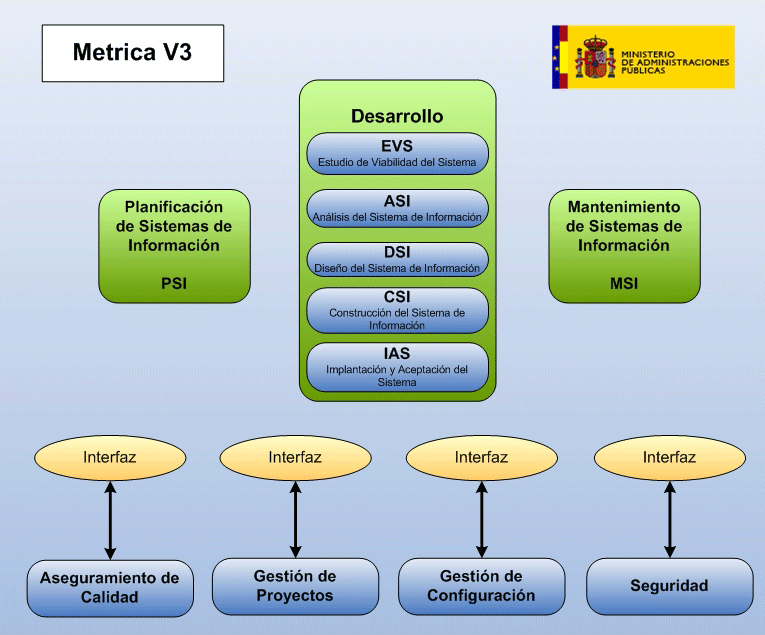
\includegraphics[scale=0.6]{Metrica3.png}}
\end{figure}

\section{Estructura del documento}
En esta sección se presentan los diferentes capítulos que conforman este documento, para que se puedan entender mejor las diferentes fases de Métrica V3 que completan el ciclo de desarrollo del proyecto. 

Capítulos en los que se divide el documento:

\begin{itemize}
    \item \textbf{Introducción (\autoref{ch:introduccion}):} Este capítulo tiene como propósito presentar al lector el tema que se tratará antes de profundizar en él. También se presentan las motivaciones que se han tenido en cuenta para la elección de este tema y los objetivos de este TFG. Por último, se explica la estructura y metodología que sigue el contenido. 
    \item \textbf{Estado del arte (\autoref{ch:estado}):} Consiste en un análisis de la situación actual del producto que planeamos desarrollar, buscando soluciones existentes al problema que intentamos solucionar o que sean similares. Después de conocer esas soluciones se buscan los puntos fuertes para intentar mejorarlos y los débiles para solucionarlos, para sacar el mejor producto posible al mercado.
    \item \textbf{Análisis del sistema - ASI (\autoref{ch:analisis}):} Presenta las especificaciones del sistema que el cliente ha solicitado, así como los casos de uso, las diferentes situaciones en las que se podrá interactuar con el mismo. Las especificaciones se recogerán como requisitos de usuario, que tras haber sido analizadas por el analista se completaran y especificaran mejor en forma de requisitos funcionales y no funcionales. Para comprobar que todo ha sido recogido correctamente se verificara con matrices de trazabilidad.
    \item \textbf{Diseño del sistema - DSI (\autoref{ch:diseno}):} 
    \item \textbf{Implementación - CSI (\autoref{ch:implementacion}):} 
    \item \textbf{Pruebas (\autoref{ch:pruebas}):} Se especifican cuáles serán las pruebas que se realizarán para comprobar que el sistema funciona correctamente, además de garantizar que se cumplen todas las especificaciones marcadas por el cliente en los requisitos del análisis.
    \item \textbf{Gestión del proyecto - PSI (\autoref{ch:gestion}):} Expone la planificación temporal del proyecto, indicando el tiempo dedicado a cada una de las partes del documento, acompañado del diagrama de Gantt correspondiente. \\ Este capítulo también comprende el presupuesto, en el que se presentan de manera desglosada todos los gastos asociados al proyecto, y finaliza con un resumen en el que se indica el precio final del proyecto para nuestro cliente.
    \item \textbf{Marco regulador (\autoref{ch:marco}):} Recoge los aspectos legales relacionados con el proyecto, con las tecnologías que se han empleado y el impacto de nuestro sistema.
    \item \textbf{Conclusiones (\autoref{ch:conclusiones}):} Es el último capítulo del desarrollo del proyecto, en el que se recoge, tras todo el proceso de diseño e implementación, cuáles son las virtudes de este sistema, así como mi valoración personal sobre el conjunto de este trabajo. \\ Se concluye con una mirada al futuro, con posibles aplicaciones que se le podrán dar y analizando cuáles serían posibles mejoras y funcionalidades para el producto. 
    \item \textbf{Bibliografía:} Recoge las referencias a todos los recursos que han sido consultados durante la realización de este documento, con el propósito de dar validez a la información que se ha presentado y si fuera necesario profundizar más en algún punto.
\end{itemize}